\documentclass[a4paper, oneside, final]{article}
\usepackage[T1]{fontenc}
\usepackage[utf8]{inputenc}
\usepackage[british]{babel}
\usepackage{amsmath}
\usepackage{amsthm}
\usepackage{verbatim}
\usepackage{listings}


\lstset{
  language=Haskell, 
  frame=tb, 
  basicstyle=\footnotesize
}


\renewcommand{\britishhyphenmins}{22} 

\let\fref\undefined
\let\Fref\undefined

\usepackage{graphicx}
\usepackage{amssymb}

\setcounter{secnumdepth}{1} % Sæt overskriftsnummereringsdybde. Disable = -1.
\setlength{\parskip}{0.25in}

\pagestyle{plain}

\title{The Par monad with distributed heaps \newline \large{Topics in Programming Languages}}
\author{Troels Henriksen \& Mads Hartmann Jensen}

\begin{document}

\maketitle

\section{Abstract}

After many false starts throughout the past twenty years, physical
laws are finally forcing parallel computers into the mainstream.  This
creates many challenges for programmers accustomed to sequential
programming, but also motivation for developing new techniques.
Functional parallel programming is an application of classical
functional programming techniques, such as higher-order functions and
purity, to the problem of parallelism.  In Haskell, the \textit{Par
  monad} (covered in detail in section \ref{sec:parmonad}) is an
abstract programming interface for doing parallel computing based on
write-once communication variables.  Unfortunately, the common
implementation of the Par monad is fundamentally based on running
multiple threads within a single operating system process, which means
that the program cannot take advantage of more than one physical
machine.  Eden (covered in detail in section \ref{sec:eden}) is an
implementation of a \textit{distributed heap} for Haskell, that makes
it possible to distribute a Haskell program across an entire network
of machines.  We present an implementation of the Par monad that makes
use of the distributed heap provided by Eden, and demonstrate how
unchanged programs can now run on cluster computers.

\newpage 

\section{Eden}
\label{sec:eden}

Eden is a parallel functional programming language which extends
Haskell with constructs for the definition and instantiation of
parallel processes. Eden has been designed for distributed-memory
machines, i.e. clusters, this means that it is based on 
message-passing. This paradigm is very suitable for functional
programming and, as it turns out, very suitable for the Par Monad
as well. 

As mentioned Eden uses the process abstraction to provide parallelism.
The two main functions are \texttt{process} and \texttt{\#}. The
\texttt{process} functions turns a regular function into a parallel
processes and \texttt{\#} instantiates the parallel process with the
given argument and returns its result. \newline 

\begin{lstlisting}
process :: ( Trans a , Trans b ) => (a -> b) -> Process a b
( # )   :: ( Trans a , Trans b ) => Process a b -> a -> b
\end{lstlisting}

These two functions are all you need to write parallel programs using
Eden. The example below shows a parallel implementation of the
Fibonacci sequence. \newline

\begin{lstlisting}
fib :: Int -> Int
fib 0 = 1
fib 1 = 1
fib n = process fib # (n-1) + process fib # (n-2)
\end{lstlisting}

Eden also provides a variety of skeletons for parallel processing
tasks that makes it faster to write parallel programs. However, in
our case both the process abstraction and the skeletons are too 
high-level for our need as we're mainly interested in the distributed
heap. Instead we use EDI, the Eden Implementation Language, to
implement the Par Monad.

\subsection{EDI}
\label{sub:edi}

At the EDI level of Eden we deal with channels. Each Eden channel
connects an outport of the sender process to an inport of the receiver
process. Each machine runs a process, consisting of multiple threads,
with a one-to-one relation between threads and outports. Each thread
of a process evaluates some expression to normal form and sends the
result via its outport. In the type-system a channel is represented as
\texttt{ChanName} with three integers used to identify the inport
connecting a channel with a process. \newline

\begin{lstlisting}
data ChanName' a = Chan Int# Int# Int#
data Mode = Connect | Stream | Data | Instantiate Int

createC :: IO ( ChanName' a, a ) 
connectToPort :: ChanName' a -> IO ()
sendData :: Mode -> a -> IO ()
spawnProcessAt :: Int -> IO () -> IO ()
sendWith :: Strategy a -> ChanName' a -> a -> IO ()
\end{lstlisting}

The function \texttt{createC} creates a primitive input channel and a
handle to access the data received via this channel. The handle is
simply represented as a normal Haskell value, however, when you try to
access the value the RST will block until it has retrieved a value via
the channel. In other words there are no primitives for reading data
as this is done implicitly by the runtime system which writes data
received via an inport directly into the placeholder in the heap.
\texttt{connectToPort} connects the outport of the thread executing
the function call to a given channel i.e. the corresponding inport.
When using \texttt{sendData} you pass a mode as well as the data to be
transmitted. The \texttt{Connect} \texttt{Mode} is initially sent to
connect the outport to the corresponding inport. the \texttt{Data
Mode} is used to send a single value whereas \texttt{Stream} is used
to send the values of a data stream element-by-element. The
\texttt{Instantiate i} message is sent to start a remote process on
processing element i.  \texttt{spawnProcessAt} starts a given process
on a specific machine.  If you pass 0 it will use round-robin
scheduling. \texttt{sendWith}  sends a value to a channel using a
specific evaluation strategy.

This is what you need to know to understand the Par Monad
implementation. For more information about Eden please refer
to ``Eden - Parallel Functional Programming with Haskell''\cite{eden}

\section{Par Monad}
\label{sec:parmonad}

The Par Monad was originally described in the paper ``A monad for deterministic parallelism''\cite{parmonad}. As the name suggests it is a monad for specifying pure parallel computations. It is especially well suited for dataflow networks. The purpose of this section is to make the reader comfortable with the Par Monad such that the next section will be understandable.

Given a computation in the Par Monad you can execute it concurrently with the current computation using the \texttt{fork} function. Computations in the \texttt{Par} monad can be extracted using the \texttt{runPar} function. \newline

\begin{lstlisting}
fork :: Par () -> Par ()
runPar :: Par a -> a
\end{lstlisting}

The astute reader may notice that \texttt{fork} and \texttt{runPar} aren't very useful by themselves as you would never be able to read the values produced by the parallel computations. A way to communicate results from the child to the parent process is necessary; for this the Par monad uses a communication abstraction they call IVars. \texttt{IVar}'s also act as the entry point to the Par Monad. \newline

\begin{lstlisting}
data IVar a 

new :: Par (IVar a)
get :: IVar a -> Par a
put :: NFData a => IVar a -> a -> Par ()
\end{lstlisting}

The \texttt{new} function creates a new IVar, \texttt{get} reads the
value stored in the IVar and \texttt{put} writes a value to the IVar.
If you invoke \texttt{get} on an empty \texttt{IVar} it will block
until a value is stored in the \texttt{IVar}. Readers familiar with
concurrent programming in Haskell may notice that this approach is
very similar to the use of \texttt{MVar} with the main difference that
IVars are write-once where \texttt{MVar}'s can be written multiple
times.

These five functions are that is needed to write parallel programs
using the Par Monad. The following listing shows a small example
program taken from \texttt{Control.Monad.Par} on
hackage\footnote{http://hackage.haskell.org/packages/archive/monad-
par/0.1.0.1/doc/html/Control-Monad-Par.html} \newline

\begin{lstlisting}[numbers=left, numberstyle=\tiny]
runPar $ do
   [a,b,c,d] <- sequence [new,new,new,new]
   fork $ do x <- get a; put b (x+1)
   fork $ do x <- get a; put c (x+2)
   fork $ do x <- get b
             y <- get c 
             put d (x+y)
   fork $ do put a (3 :: Int)
   get d
\end{lstlisting}

On line 2 four \texttt{IVar}'s are created. Lines 3-8 creates tasks
that read and write to different IVars in parallel. Line 9 reads the
value stored in the IVar bound to d and as such this is the value
returned by the entire program.The program is shown as a data-flow
diagram below. \newline

\begin{lstlisting}
                            a
                           / \  
                          b   c
                           \ /
                            d
\end{lstlisting}

This should be sufficient to understand the purpose and usage of the
Par Monad.

\newpage

\section{Implementing the Par Monad}

Now that we've introduced EDI and the Par Monad it is time see how 
the two fit together. Our task is twofold: Figure out how to 
represent Par processes (that is, implement \texttt{runPar} and 
\texttt{fork}) and how to represent IVars using the primitive
channel operations provided by EDI.

Par processes are easily implemented using EDI \newline

\begin{lstlisting}
newtype Par a = Par { runPar :: IO a }
fork m = Par $ do spawnProcessAt 0 $ runPar m
                  return ()
\end{lstlisting}

As such the challenge lies in deciding how to represent an \texttt{IVar}
using EDI. The obvious way to would be to represent it simply as a
channel. \newline

\begin{lstlisting}
newtype IVar a = IVar (ChanName' a, a)
\end{lstlisting}

However, this value returned by \texttt{createC} is a backhole. In 
the RTS, blackholes are thunks that are currently being evaluated by
another thread. Consider the following program \newline 

\begin{lstlisting}[language=Haskell]
test :: Int -> Par Int
test x = do ivar <- new
            fork $ put ivar (x+1)
            get ivar
\end{lstlisting}

If \texttt{ivar} contains a black hole, then \texttt{fork} will block
until it has been filled, as its value has to be sent to the process
that is going to execute the IO action.  But that IO action is the one
that will fill the hole hence we have a deadlock.

Instead we represent an \texttt{IVar} as a channel for writing its
value, as well as a channel for requesting its value. \newline

\begin{lstlisting}
data IVar a = IVar { iVarReadChan :: ChanName' [ChanName' a]
                   , iVarWriteChan :: ChanName' a
                   }
\end{lstlisting}

With this definition the \texttt{get} function can be implemented as 
such: \newline

\begin{lstlisting}[numbers=left, numberstyle=\tiny]
get ivar = Par $ do
             (c,x) <- createC
             connectToPort (iVarReadChan ivar)
             sendData Stream c
             return x
\end{lstlisting}

On line 1 we create the channel from which we want to read the value
stored in the \texttt{IVar}. On line 3-4 we connect to the given
\texttt{IVar}'s read channel and send the channel we created on line 1. 
Finally we return the value \texttt{x} written to the channel created on line 1. Remember this will block until a value has actually been written to 
channel \texttt{c}.

With this approach every \texttt{IVar} now has an associated lightweight
Haskell thread that handles read requests. \newline

\begin{lstlisting}[numbers=left, numberstyle=\tiny]
new = Par $ do
        (rdc,rd) <- createC
        (wrc,wr) <- createC
        _ <- forkIO $ do
          let val = wr
              cs  = rd
          mapM_ (\c -> sendWith rseq c val) cs
        return $ IVar rdc wrc
\end{lstlisting}

On line 2 we create the channel for reading and on line 3 we create
the channel for writing the value of the  \texttt{IVar}. On lines 4 to
7 we create a lightweight Haskell thread the handles all of the read
request. Line 5 will block till a process has written a value to the
write channel. On line 6 we utilize Edens ability to transmit streams
element-by-element and handle each read request sequentially using
\texttt{mapM\_}. This fixes our blackhole problem but unfortunately
introduces a new one: The thread on lines 5 -7 never terminates as we
can't tell when to stop waiting for more read requests. If there are
no requests mapM\_ will be waiting indefinitely and as such represents
a memory leak.

\subsection{Resource leak}

I'll be writing something about the process leak here.

\section{Performance}

\begin{figure}
\caption{Parallel computation of Fibonacci numbers}
\label{fig:parfib}
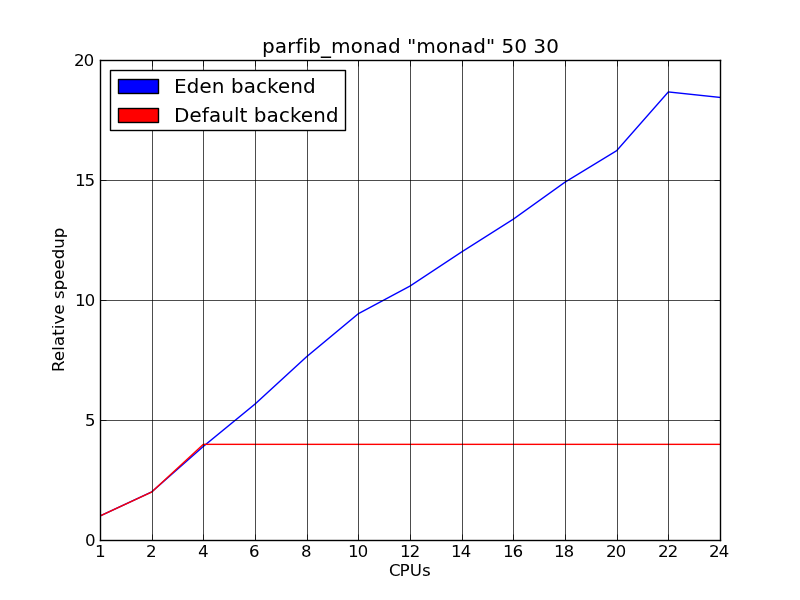
\includegraphics[width=7cm]{parfib_monad-speedup.png}
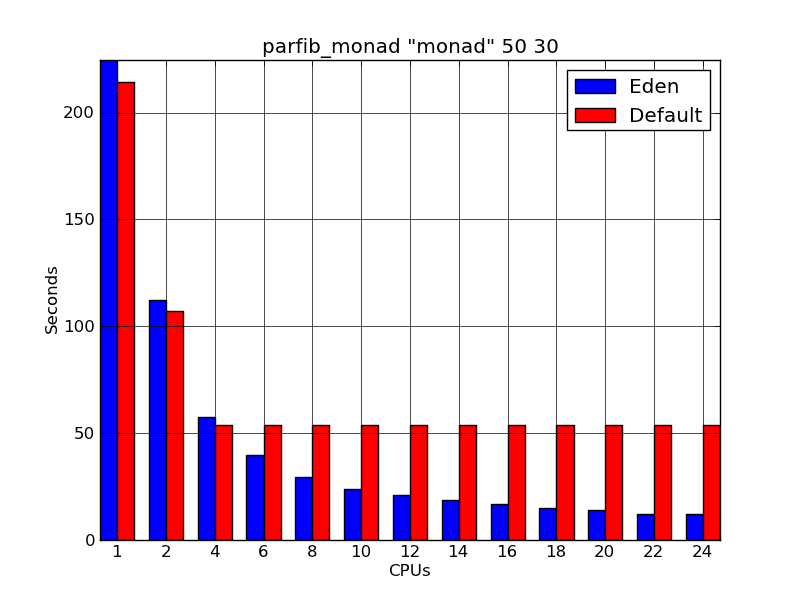
\includegraphics[width=7cm]{parfib_monad-runtimes.png}
\end{figure}

\begin{figure}
\caption{Black-Scholes}
\label{fig:blackscholes}
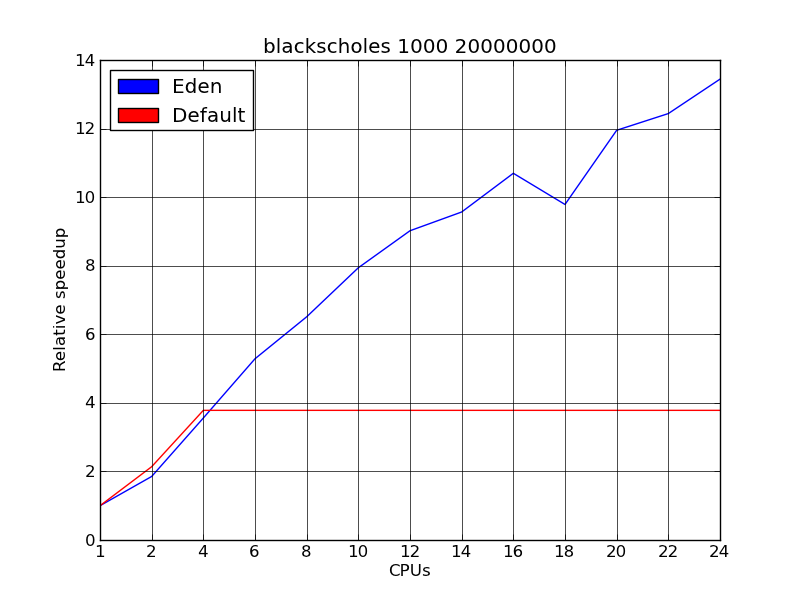
\includegraphics[width=7cm]{blackscholes-speedup.png}
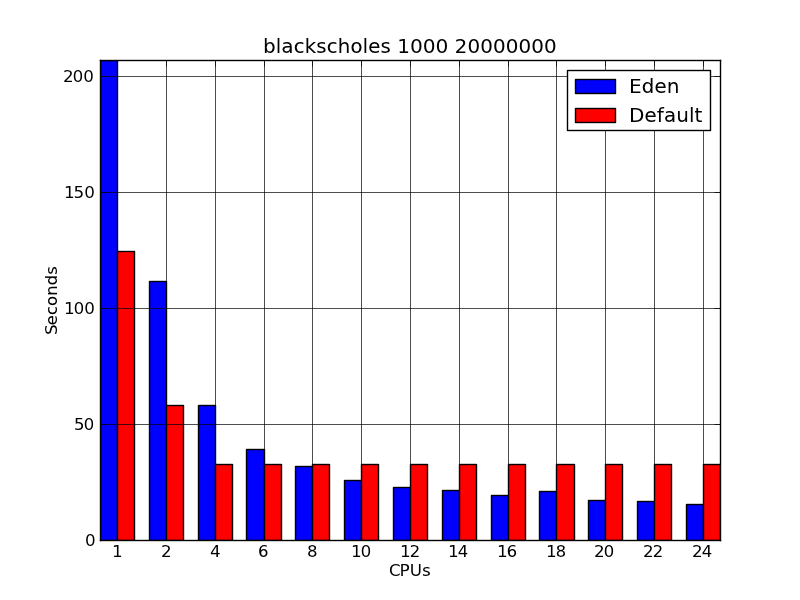
\includegraphics[width=7cm]{blackscholes-runtimes.png}
\end{figure}

\begin{figure}
\caption{N-body problem}
\label{fig:nbody}
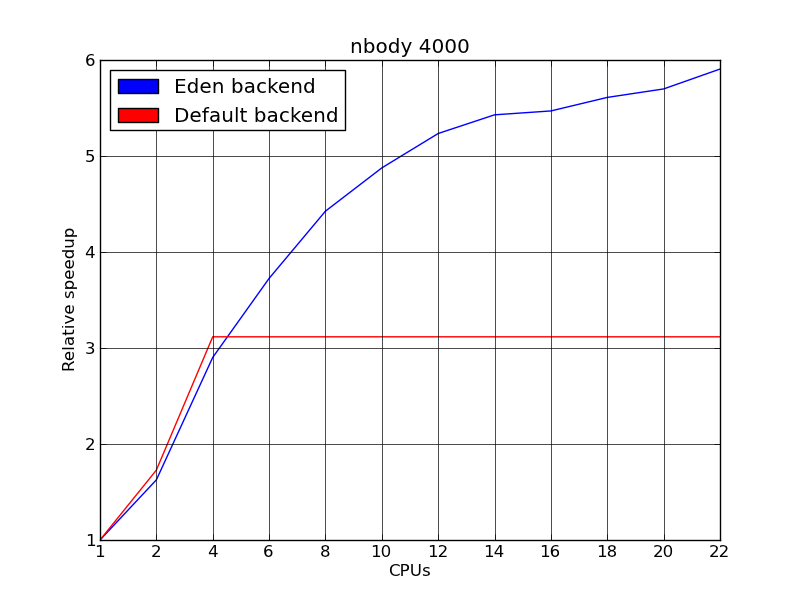
\includegraphics[width=7cm]{nbody-speedup.png}
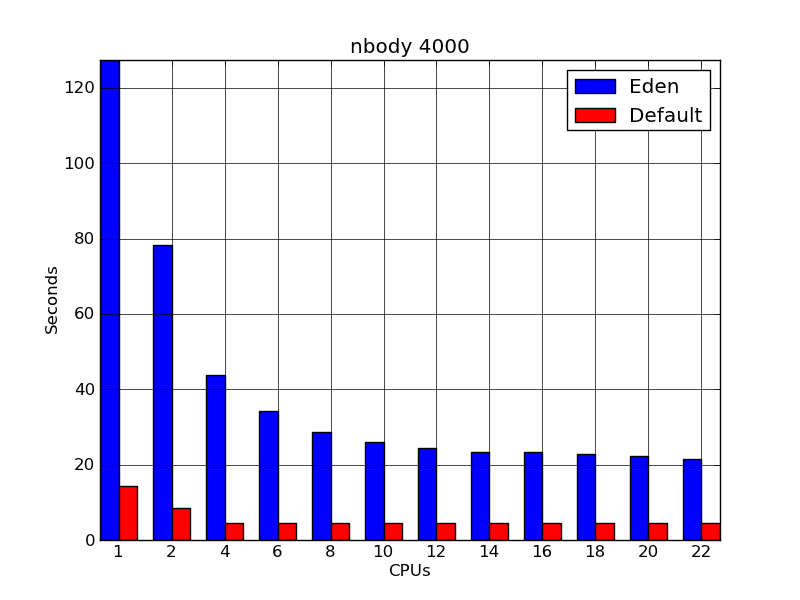
\includegraphics[width=7cm]{nbody-runtimes.png}
\end{figure}

We have performed limited benchmarking of our implementation of the
Par backend, wherein we compare our performance to the default
implementation.  Tests were performed on
$\texttt{sci-0},\texttt{sci-1},\ldots,\texttt{sci-6}$, six computation
nodes available on the DIKU network, with each running a quad-core
2.40GHz Intel Xeon processor.  The \texttt{sci} systems are
virtualised servers, resulting in unknown network topography and
system load, which has resulted in some unpredictable variation in
performance, and while we re-ran some benchmarks multiple times to
obtain sensible results, there are still some inexplicable artifacts
left.  The benchmarks are thus not a very precise indication of the
ultimate performance potential of the EDI-based Par monad, but rather
a basic demonstration of the viability of the approach.  A serious
exploration of the implementation should involve benchmarks on
dedicated cluster computing systems.  Finally, note that it is not
possible to run the default Par monad implementation in a distributed
setting, hence it does not benefit from access to more than the four
CPUs available on a single machine.  The benchmark programs have been
taken from the \texttt{monad-par} package and were unmodified.
Specific parameters have been tuned to exhibit relatively long
runtimes and sensible chunking of parallel work, so the results should
not be dominated by startup overhead, or exhibit non-realistic
workloads.

A probably best-case situation for our monad is shown in Figure
\ref{fig:parfib}.  The Parfib program computes a Fibonacci number
using the recursive formula $fib(n) = fib(n-1) + fib(n-2)$; running
the recursive calls in parallel, except when $n$ is less than a given
threshold.  In the benchmark, we compute $fib(50)$, with $n=30$ as the
threshold for switching to sequential computation, resulting in a
manageable (although still large) number of processes, each doing a
relatively work-intensive task (computing $fib(30)$).  As a
consequence, since the runtime is dominated by the actual work, the
increased overhead of EDI process creation and communication is not
very noticable, and we scale essentially linearly (except for a hiccup
at the very end, most likely due to virtualisation artifacts).

Figure \ref{fig:blackscholes} shows results from an implementation of
the Black-Scholes equation, executed with parameters corresponding to
$20,000,000$ options divided into $1000$ blocks.  We observe
almost-linear scaling, but also significant overhead.  As the core of
the benchmark program is a naïve parallel map across a list of twenty
thousand elements (one process per element), this is not particularly
surprising, given that EDI threads are somewhat heavy compared to
lightweight GHC threads.

This issue is particularly noticable in the results on Figure
\ref{fig:nbody}, which computes accelerations for an N-body system
(with $N=4000$).  The program creates an array of four thousand
floating point values, creates four thousand processes (one for each
simulated body), then waits for sums up the results.  We have
extremely fine task granularity, which means we scale well (at the
start, at least), but the overhead of creating so many threads results
in terrible performance.  There is a deeper problem, however: each
process consists of a Par action that contains a reference to the
4000-element vector, and for each process to be started on a different
machine, \textit{the entire vector is sent over the network}.  While
we could in principle send the value only once to each node, it is not
practically feasible, and Eden does not keep track of whether some
specific value has already been sent to a given node and so performs
an extremely large amount of extra work.  As a back-of-the-envelope
calculation, if we assume that each element of the vector takes up
eight bytes\footnote{The actual space consumption is likely to be much
  larger, as the N-body program uses arrays with boxed elements.}, the
entire vector takes up $4000\times8\text{B}\approx 32\text{KiB}$,
which, for the 24-CPU/six-nodes case results in $\frac{5}{6} \times
4000 \times 32\text{KiB}\approx 125\text{MiB}$ of network traffic.
Also, since the first process, which is responsible for creating the
four thousand worker processes, is also responsible for sending these
vectors, it acts as a bottleneck when we try to scale upwards.  The
default Par monad implementation needs to do no copying when sharing
data with new processes, and so does not suffer from this problem.

\section{Conclusions}

It is possible to implement the Par monad on top of the distributed
heap provided by Eden, although the mapping of \texttt{IVar}s to Eden
channels requires nontrivial work to solve a resource leak problems.

Our implementation of the Par monad is able to scale well across a
distributed system, although its performance characteristics differ
from the default Par monad implementation.  Notably, processes are far
more expensive, and reading an \texttt{IVar} containing a large object
may involve heavy network traffic.  This seems a fundamental problem
with the idea of providing a common parallel programming interface -
some measure of the cost of underlying abstractions must be available
for sensible workload chunking to be possible, as parallel hardware is
too diverse for an practical abstract cost model to be available the
way it is for sequential programming.

\subsection{Ideas for further work}

Our implementation is a very thin layer on top of the EDI primitives.
An interesting project would be the implementation of a more
sophisticated scheduler that tries to keep network traffic to a
minimum, by keeping communicating threads on the same physical node
(and perhaps does not even spawn physical EDI threads until
necessary).  Haskell threads are extremely flexible due to their light
weight, yet our implementation makes little use of them.

\bibliography{report}

\end{document}
